% !TEX root = ../tex/5-3.tex
% 第5章：本文は青、補足は緑
\newcommand{\asmain}{%
    \setbeamercolor{frametitle}{fg=white,bg=main}%
    \setbeamercolor{structure}{fg=main}%
    \setbeamercolor{itemize item}{fg=main}%
    \setbeamercolor{itemize subitem}{fg=main}%
    \setbeamercolor{enumerate item}{fg=main}%
}
\newcommand{\assuppl}{%
    \setbeamercolor{frametitle}{fg=white,bg=examplecol}%
    \setbeamercolor{structure}{fg=examplecol}%
    \setbeamercolor{itemize item}{fg=examplecol}%
    \setbeamercolor{itemize subitem}{fg=examplecol}%
    \setbeamercolor{enumerate item}{fg=examplecol}%
}
% フレームタイトルの「補足」だけを□で囲む
\newcommand{\supplmark}{%
    \setlength{\fboxsep}{1.5pt}%
    \setlength{\fboxrule}{0.7pt}%
    \fbox{\textbf{補足}}%
}
\asmain


%=============================================
\begin{frame}{5.2から5.3へ}
    \begin{block}{ここまで（5.2）}
        Flow Matchingは、周辺速度$v_t$を学習目標にする。\\
        ただし一般分布では$v_t$が未知なので、\\
        Conditional Flow Matching（CFM）で\\
        条件付き速度$v_t(\cdot|z)$を代理教師にする。
    \end{block}
    \begin{block}{ここから（5.3）}
        $p_t(\cdot|z)$と$v_t(\cdot|z)$をどう設計するか。\\
        ガウス橋を雛形に、\\
        \textbf{path-first}と\textbf{flow-first}の2つの作り方を見る。
    \end{block}
\end{frame}
%=============================================
\asmain
\begin{frame}{5.3 の位置づけ}
    \begin{block}{この節の役割}
        任意の端点分布をつなぐ、扱いやすい条件付き過程を構成する
    \end{block}
    \begin{enumerate}
        \item \textbf{5.3.1 ガウス橋}\\
        周辺$p_t$と速度$v_t$が閉じた形で書ける特殊例
        \item \textbf{5.3.2 Path-first}\\
        条件付き密度$p_t(\cdot|z)$を先に置き、$v_t(\cdot|z)$を導く
        \item \textbf{5.3.3 Flow-first}\\
        条件付きフロー$\Psi_{0\to t}(\cdot|z)$を先に置く
        \item \textbf{5.3.4 比較}\\
        Euler / Lagrange、一意性、使いどころ
        \item \textbf{5.3.5 直線性}\\
        条件付き直線 $\neq$ 周辺ODEの直線
    \end{enumerate}
\end{frame}
%=============================================
\section{5.3.1 ガウス橋}
\asmain
\begin{frame}{区切り：5.3.1 ガウス橋}
    \tableofcontents[currentsection]
\end{frame}
%=============================================
\asmain
\begin{frame}{なぜガウス橋から始めるか}
    CFMでは、条件付き過程が次を満たす必要がある。
    \begin{itemize}
        \item $p_t(\cdot|z)$から効率よくサンプルできる
        \item $v_t(\cdot|z)$が閉じた式で書ける
    \end{itemize}
    \begin{block}{完全に解ける例}
        端点がともにガウスなら、周辺密度と速度が解析的に求まる。\\
        これが一般の条件付き構成の雛形になる。
    \end{block}
\end{frame}
%=============================================
\asmain
\begin{frame}{ガウス密度パス}
    平均$\mu(t)$・分散$\sigma^{2}(t)>0$のガウスパス：
    \[
        p_t(\bm{x}_t)
        =
        \mathcal{N}\!\bigl(\bm{x}_t;\,\mu(t),\,\sigma^{2}(t)\bm{I}\bigr)
        \tag{5.3.1}
    \]
    端点は
    \[
        p_{\mathrm{src}}=p_0=\mathcal{N}(\mu(0),\sigma^{2}(0)\bm{I}),
        \quad
        p_{\mathrm{tgt}}=p_1=\mathcal{N}(\mu(1),\sigma^{2}(1)\bm{I}).
    \]
    \begin{exampleblock}{注意}
        同じ$\{p_t\}$を生む速度場は一般に一意ではない。\\
        ここでは単純なアフィンフローを1つ選ぶ。
    \end{exampleblock}
\end{frame}
%=============================================
\asmain
\begin{frame}{アフィンフローと閉じた速度}
    正規化したアフィンフロー：
    \[
        \Psi_{0\to t}(\bm{x})
        :=
        \mu(t)+\sigma(t)\dfrac{\bm{x}-\mu(0)}{\sigma(0)}
        \tag{5.3.2}
    \]
    \begin{block}{命題5.3.1（閉じた速度）}
        この$\Psi_{0\to t}$を誘導する速度は一意で、
        \[
            v_t(\bm{x})
            =
            \dfrac{\sigma'(t)}{\sigma(t)}\bigl(\bm{x}-\mu(t)\bigr)
            +
            \mu'(t).
        \]
    \end{block}
\end{frame}
%=============================================
\assuppl
\begin{frame}{\supplmark：命題5.3.1の導出スケッチ}
    フロー定義のODE：
    \[
        \dfrac{d}{dt}\Psi_{0\to t}(\bm{y})
        =
        v_t\bigl(\Psi_{0\to t}(\bm{y})\bigr).
    \]
    $\sigma(t)>0$より$\Psi_{0\to t}$は可逆なので、
    $\bm{x}=\Psi_{0\to t}(\bm{y})$とおくと
    \[
        v_t(\bm{x})
        =
        \bigl(\partial_t\Psi_{0\to t}\bigr)
        \circ
        \Psi_{0\to t}^{-1}(\bm{x}).
    \]
    \begin{exampleblock}{要点}
        flow-firstなら速度は一意。\\
        path-firstだけだと、連続方程式を満たす速度は一般に非一意。
    \end{exampleblock}
\end{frame}
%=============================================
\asmain
\begin{frame}{5.3.1 のまとめ}
    \begin{itemize}
        \item ガウスパス（5.3.1）＋アフィンフロー（5.3.2）で速度が閉じる
        \item $v_t(\bm{x})=\frac{\sigma'}{\sigma}(\bm{x}-\mu)+\mu'$（命題5.3.1）
        \item この形は、条件付き$z$を入れてもそのまま使える雛形である
    \end{itemize}
    \begin{block}{次}
        一般端点へ拡張し、条件付きpathを先に置く構成を見る。
    \end{block}
\end{frame}
%=============================================
\section{5.3.2 Path-first}
\asmain
\begin{frame}{区切り：5.3.2 Path-first}
    \tableofcontents[currentsection]
\end{frame}
%=============================================
\asmain
\begin{frame}{条件付き過程の2タイプ}
    条件変数$z\sim\pi$の取り方で、よく使うのは次の2つ。
    \begin{columns}[T,onlytextwidth]
        \begin{column}{0.48\textwidth}
            \begin{block}{Two-sided}
                $z=(\bm{x}_0,\bm{x}_1)$\\
                「ビーム型」パス
            \end{block}
        \end{column}
        \begin{column}{0.48\textwidth}
            \begin{block}{One-sided}
                $z=\bm{x}_0$または$\bm{x}_1$\\
                「スポットライト型」パス
            \end{block}
        \end{column}
    \end{columns}
    \vfill
    どちらも境界で
    \[
        p_{\mathrm{src}}=\int p_0(\cdot|z)\pi(z)\,dz,
        \quad
        p_{\mathrm{tgt}}=\int p_1(\cdot|z)\pi(z)\,dz
    \]
    を満たす必要がある。
\end{frame}
%=============================================
\asmain
\begin{frame}{図5.9：条件付きパスの型}
    \centering
    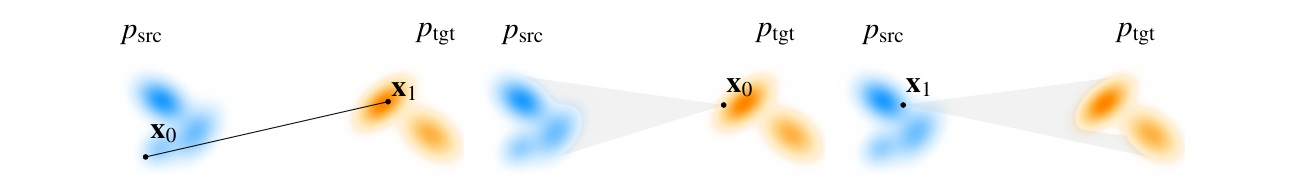
\includegraphics[width=\textwidth,height=0.55\textheight,keepaspectratio]{fig-5-9.jpg}
    \vfill
    左：両端$(\bm{x}_0,\bm{x}_1)$で条件付け（ビーム）。\\
    中・右：片側だけ条件付け（スポットライト）。
\end{frame}
%=============================================
\assuppl
\begin{frame}{\supplmark：図5.9の読み方}
    \begin{exampleblock}{左：two-sided}
        固定した$(\bm{x}_0,\bm{x}_1)$をつなぐ細い経路。\\
        独立サンプル対$\pi(z)=p_{\mathrm{src}}(\bm{x}_0)p_{\mathrm{tgt}}(\bm{x}_1)$が典型。
    \end{exampleblock}
    \begin{exampleblock}{中・右：one-sided}
        片方の点を固定し、もう一方の分布全体へ広がる／集まる。\\
        生成設定では$z=\bm{x}_1\sim p_{\mathrm{data}}$が多い。
    \end{exampleblock}
\end{frame}
%=============================================
\asmain
\begin{frame}{Two-sided：ビーム型パス}
    $\pi(z)=p_{\mathrm{src}}(\bm{x}_0)p_{\mathrm{tgt}}(\bm{x}_1)$とし、
    \[
        p_t(\bm{x}_t|z)
        =
        \mathcal{N}\!\bigl(
            \bm{x}_t;\,
            a_t\bm{x}_0+b_t\bm{x}_1,\,
            \sigma^{2}\bm{I}
        \bigr)
    \]
    （$a_0=1,b_0=0$、$a_1=0,b_1=1$；典型は$a_t=1-t$、$b_t=t$）。
    \begin{block}{条件付き速度（命題5.3.1）}
        \[
            v_t(\bm{x}|z)=a_t'\bm{x}_0+b_t'\bm{x}_1
        \]
        （分散が時間一定ならスケール項は消える）
    \end{block}
\end{frame}
%=============================================
\asmain
\begin{frame}{Two-sided CFM損失}
    $\sigma=0$なら$\bm{x}_t=a_t\bm{x}_0+b_t\bm{x}_1$で、
    \[
        \mathcal{L}_{\mathrm{CFM}}
        =
        \mathbb{E}_{t,\bm{x}_0,\bm{x}_1}
        \bigl\|
            v_\phi(\bm{x}_t,t)
            -
            (a_t'\bm{x}_0+b_t'\bm{x}_1)
        \bigr\|_{2}^{2}.
    \]
    \begin{block}{最適解}
        \[
            v^{\star}(\bm{x}_t,t)
            =
            \mathbb{E}\bigl[a_t'\bm{x}_0+b_t'\bm{x}_1\bigm|\bm{x}_t\bigr]
        \]
        （$\bm{x}_t$を生み得た端点対の事後期待値）
    \end{block}
\end{frame}
%=============================================
\asmain
\begin{frame}{One-sided：スポットライト型}
    $z=\bm{x}_1\sim p_{\mathrm{data}}$、$p_{\mathrm{src}}=\mathcal{N}(\bm{0},\bm{I})$として
    \[
        p_t(\bm{x}_t|\bm{x}_1)
        =
        \mathcal{N}\!\bigl(\bm{x}_t;\,b_t\bm{x}_1,\,a_t^{2}\bm{I}\bigr).
    \]
    境界は$p_0(\cdot|\bm{x}_1)=\mathcal{N}(\bm{0},\bm{I})$、$p_1=\delta(\cdot-\bm{x}_1)$。
    \begin{block}{条件付き速度}
        \[
            v_t(\bm{x}|\bm{x}_1)
            =
            b_t'\bm{x}_1
            +
            \dfrac{a_t'}{a_t}\bigl(\bm{x}-b_t\bm{x}_1\bigr)
        \]
    \end{block}
\end{frame}
%=============================================
\asmain
\begin{frame}{One-sided CFMとtwo-sidedの同値}
    損失（5.3.3）：
    \[
        \resizebox{0.98\textwidth}{!}{$
        \mathcal{L}_{\mathrm{CFM}}
        =
        \mathbb{E}_{t,\bm{x}_1}
        \mathbb{E}_{\bm{x}_t\sim p_t(\cdot|\bm{x}_1)}
        \Bigl\|
            v_\phi(\bm{x}_t,t)
            -
            \bigl(
                b_t'\bm{x}_1
                +
                \tfrac{a_t'}{a_t}(\bm{x}_t-b_t\bm{x}_1)
            \bigr)
        \Bigr\|_{2}^{2}
        $}
    \]
    対$(\bm{x}_0,\bm{x}_1)$で$\bm{x}_t=a_t\bm{x}_0+b_t\bm{x}_1$なら、
    \[
        v_t(\bm{x}_t|\bm{x}_1)=a_t'\bm{x}_0+b_t'\bm{x}_1.
    \]
    よってone-sidedとtwo-sidedの最小解は同じ$v^{\star}$。
\end{frame}
%=============================================
\asmain
\begin{frame}{Gaussian FMと拡散の接続}
    FM規約：$t=0$がsource/prior、$t=1$がtarget/data。\\
    条件付きパスがガウスなら\textbf{Gaussian FM}と呼ぶ。
    \begin{itemize}
        \item 拡散の確率パスは、その重要な部分クラス
        \item 任意のガウス日程が前向きSDEになるとは限らない\\
        （補題4.5.1の適合条件が要る）
        \item $a_t=1-t$、$b_t=t$はFM/RFの標準スケジュール
    \end{itemize}
    \begin{exampleblock}{実務}
        損失$\mathbb{E}\|v_\phi(\bm{x}_t,t)-(\bm{x}_1-\bm{x}_0)\|_{2}^{2}$は単純で、\\
        大規模でも競争力がある（Esser et al., 2024）。
    \end{exampleblock}
\end{frame}
%=============================================
\asmain
\begin{frame}{表5.2：補間係数の一覧}
    \centering
    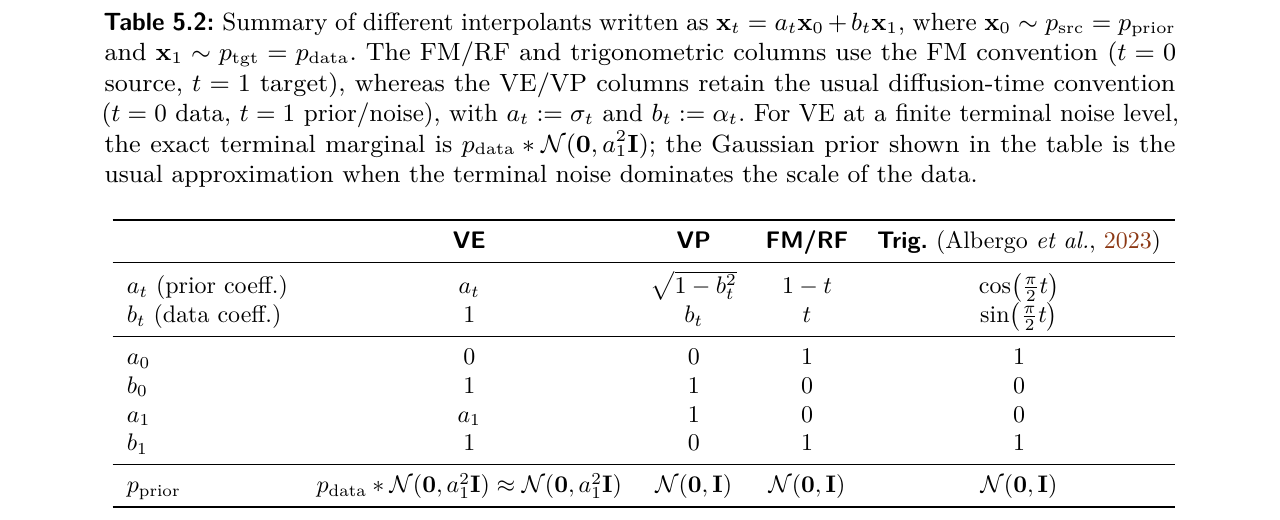
\includegraphics[width=\textwidth,height=0.72\textheight,keepaspectratio]{table-5-2.png}
\end{frame}
%=============================================
\assuppl
\begin{frame}{\supplmark：表5.2の読み方}
    \begin{itemize}
        \item すべて$\bm{x}_t=a_t\bm{x}_0+b_t\bm{x}_1$の形
        \item FM/RF・Trig.はFM時間（$0$=source、$1$=target）
        \item VE/VP列は拡散時間（$0$=data、$1$=prior）のまま
        \item FM/RF列$a_t=1-t$、$b_t=t$が「直線補間」の標準
    \end{itemize}
    \begin{exampleblock}{第6章への伏線}
        Gaussian FMは、線形日程のもとで\\
        速度予測型の拡散と等価に読める。
    \end{exampleblock}
\end{frame}
%=============================================
\asmain
\begin{frame}{5.3.2 のまとめ}
    \begin{itemize}
        \item Path-first：まず$p_t(\cdot|z)$を置き、命題5.3.1で$v_t(\cdot|z)$を得る
        \item Two-sidedはビーム、one-sidedはスポットライト（図5.9）
        \item 両者のCFM最適解は一致し、Gaussian FMは拡散と接続する
    \end{itemize}
    \begin{block}{次}
        密度ではなくフロー写像を先に置く構成（flow-first）。
    \end{block}
\end{frame}
%=============================================
\section{5.3.3 Flow-first}
\asmain
\begin{frame}{区切り：5.3.3 Flow-first}
    \tableofcontents[currentsection]
\end{frame}
%=============================================
\asmain
\begin{frame}{なぜフローを先に置くか}
    任意端点$p_{\mathrm{src}}$、$p_{\mathrm{tgt}}$に対し、\\
    軌跡空間で条件付きフロー$\Psi_{0\to t}(\cdot;z)$を直接指定する。
    \begin{block}{利点}
        \begin{itemize}
            \item 軌跡の時間微分が、そのまま回帰教師になる
            \item 多様体・Lie群などでは測地線／指数写像が自然
            \item シミュレーション不要の解析的目標速度が得られる
        \end{itemize}
    \end{block}
\end{frame}
%=============================================
\asmain
\begin{frame}{条件付きアフィンフロー}
    $z\sim\pi$を固定し、
    \[
        \Psi_{0\to t}(\bm{x}_0;z)
        :=
        \mu_t(z)+A_t(z)\bm{x}_0,
        \qquad t\in[0,1].
    \]
    境界$A_0=I$、$\mu_0=\bm{0}$で$t=0$は$p_{\mathrm{src}}$を回復。\\
    $t\to 1$は極限として解釈（特異でもよい）。
    \begin{block}{誘導されるパス}
        \[
            p_t(\cdot|z)=\Psi_{0\to t}(\cdot;z)_{\#}\,p_{\mathrm{src}}
        \]
        サンプルは$z\sim\pi$、$\bm{x}_0\sim p_{\mathrm{src}}$、$\bm{x}_t=\mu_t(z)+A_t(z)\bm{x}_0$。
    \end{block}
\end{frame}
%=============================================
\asmain
\begin{frame}{フローから速度へ}
    可逆なとき、Euler速度は
    \[
        v_t(\bm{x}|z)
        =
        \partial_t\Psi_{0\to t}(\bm{y};z)
        \Big|_{\bm{y}=\Psi_{0\to t}^{-1}(\bm{x};z)}.
    \]
    アフィンなら$\bm{x}_0=A_t(z)^{-1}(\bm{x}-\mu_t(z))$より
    \[
        v_t(\bm{x}|z)
        =
        \mu_t'(z)
        +
        A_t'(z)A_t(z)^{-1}\bigl(\bm{x}-\mu_t(z)\bigr).
    \]
    \begin{exampleblock}{注意}
        $p_{\mathrm{src}}$が非ガウスなら、アフィンフローでも$p_t(\cdot|z)$は一般に非ガウス。
    \end{exampleblock}
\end{frame}
%=============================================
\asmain
\begin{frame}{特殊化：one-sided / two-sided}
    $\mu_t(z)=b_t z$、$A_t(z)=a_t I$とすると
    \[
        \bm{x}_t=a_t\bm{x}_0+b_t\bm{x}_1,
        \qquad
        v_t(\bm{x}|\bm{x}_1)
        =
        b_t'\bm{x}_1+\tfrac{a_t'}{a_t}(\bm{x}-b_t\bm{x}_1).
    \]
    対サンプルでは再び$v_t=a_t'\bm{x}_0+b_t'\bm{x}_1$。
    \begin{block}{ガウスパスの回収}
        $\mu_t$が$z$に依らず、$A_t=\frac{\sigma(t)}{\sigma(0)}I$なら\\
        命題5.3.1のガウスパス・閉じた速度に戻る。
    \end{block}
\end{frame}
%=============================================
\asmain
\begin{frame}{5.3.3 のまとめ}
    \begin{itemize}
        \item Flow-firstは$\Psi_{0\to t}$を先に置き、pushforwardで$p_t$を得る
        \item 可逆なら$v_t=\partial_t\Psi\circ\Psi^{-1}$が一意
        \item アフィン特殊化は、path-firstの標準CFM目標と同じ式に落ちる
    \end{itemize}
    \begin{block}{次}
        2つの構成を軸ごとに比較する（表5.3）。
    \end{block}
\end{frame}
%=============================================
\section{5.3.4 Path-first vs Flow-first}
\asmain
\begin{frame}{区切り：5.3.4 比較}
    \tableofcontents[currentsection]
\end{frame}
%=============================================
\asmain
\begin{frame}{EulerとLagrange}
    \begin{columns}[T,onlytextwidth]
        \begin{column}{0.48\textwidth}
            \begin{block}{Path-first（Euler）}
                密度パス$p_t(\cdot|z)$を先に指定。\\
                連続方程式を満たす$v_t$を選ぶ。\\
                一般に速度は非一意。
            \end{block}
        \end{column}
        \begin{column}{0.48\textwidth}
            \begin{block}{Flow-first（Lagrange）}
                フロー$\Psi_{0\to t}(\cdot|z)$を先に指定。\\
                密度はpushforward。\\
                可逆ならEuler速度は一意。
            \end{block}
        \end{column}
    \end{columns}
    \vfill
    どちらも同じ種類の輸送対象を、出発点を変えて記述する。\\
    ただし「先に置いた密度」と「別途置いたフロー」が\\
    同じ速度を選ぶとは限らない。
\end{frame}
%=============================================
\asmain
\begin{frame}{表5.3：構成の比較}
    \centering
    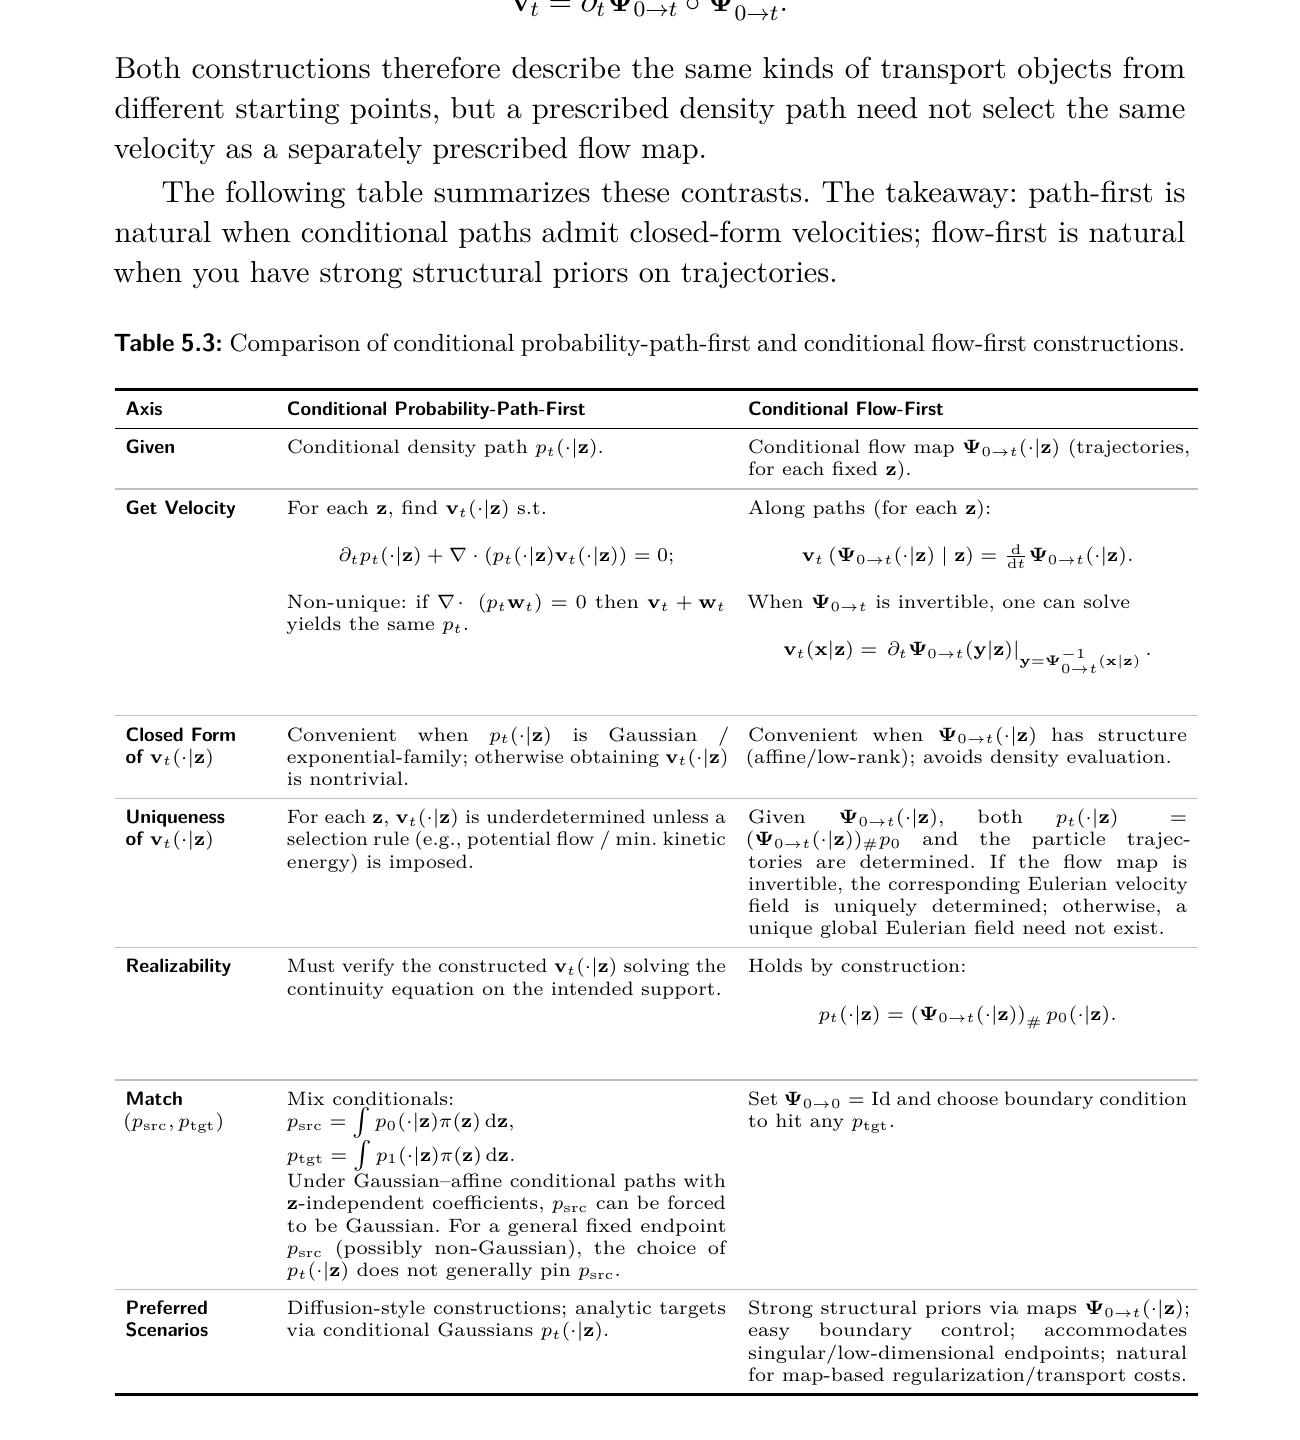
\includegraphics[width=\textwidth,height=0.72\textheight,keepaspectratio]{table-5-3.png}
\end{frame}
%=============================================
\asmain
\begin{frame}{使いどころの要約}
    \begin{block}{Path-firstが自然}
        条件付きガウスなど、閉じた速度がすぐ書けるとき。\\
        拡散型の構成と相性が良い。
    \end{block}
    \begin{block}{Flow-firstが自然}
        軌跡に強い構造事前があるとき（アフィン、測地線など）。\\
        境界制御がしやすく、特異／低次元端点も扱いやすい。
    \end{block}
    \begin{exampleblock}{実務の指針}
        「閉じた$v_t$が欲しい」ならpath-first、\\
        「軌跡の形を決めたい」ならflow-first。
    \end{exampleblock}
\end{frame}
%=============================================
\asmain
\begin{frame}{5.3.4 のまとめ}
    \begin{itemize}
        \item Path-first：密度$\to$連続方程式$\to$速度（非一意）
        \item Flow-first：フロー$\to$pushforwardと$v_t=\partial_t\Psi\circ\Psi^{-1}$（可逆なら一意）
        \item 出発点が違うだけで、同じ輸送を記述できる
    \end{itemize}
\end{frame}
%=============================================
\section{5.3.5 直線性の落差}
\asmain
\begin{frame}{区切り：5.3.5 条件付き直線 $\neq$ 周辺直線}
    \tableofcontents[currentsection]
\end{frame}
%=============================================
\asmain
\begin{frame}{条件付き直線は魅力的だが}
    標準アフィン補間
    \[
        \bm{x}_t=(1-t)\bm{x}_0+t\bm{x}_1
    \]
    は、固定$(\bm{x}_0,\bm{x}_1)$では直線・定速$\bm{x}_1-\bm{x}_0$。\\
    FM／Rectified Flowでよく使う幾何である。
    \begin{alertblock}{混同しやすい点}
        学習に使う条件付きパスが直線でも、\\
        生成時の周辺ODE軌跡が直線とは限らない。
    \end{alertblock}
\end{frame}
%=============================================
\asmain
\begin{frame}{周辺最適速度は事後平均}
    カップリング$\pi(\bm{x}_0,\bm{x}_1)$のもと、
    \[
        v^{\star}(\bm{x},t)
        =
        \mathbb{E}\bigl[\bm{x}_1-\bm{x}_0\bigm|\bm{x}_t=\bm{x}\bigr].
    \]
    端点対の事後は$(\bm{x},t)$で変わる。\\
    よって周辺ODEに沿った速度は、一般に定速ではない。
    \begin{block}{帰結}
        アフィン日程だけでは「1 Eulerステップ厳密」にはならない。\\
        Rectified FlowのReflowは、カップリングを直して\\
        因果フローを直線に近づけていく手続きである。
    \end{block}
\end{frame}
%=============================================
\asmain
\begin{frame}{1次元の反例（要旨）}
    $\bm{x}_0\sim\mathcal{N}(0,\sigma_0^{2})$、$\bm{x}_1\sim\mathcal{N}(0,\sigma_1^{2})$独立、\\
    $\bm{x}_t=(1-t)\bm{x}_0+t\bm{x}_1$とする。
    \[
        V(t)=(1-t)^{2}\sigma_0^{2}+t^{2}\sigma_1^{2},
        \quad
        v^{\star}(x,t)=\dfrac{V'(t)}{2V(t)}\,x.
    \]
    周辺ODEの解は
    \[
        z_t
        =
        z_0\sqrt{(1-t)^{2}+\bigl(\tfrac{\sigma_1}{\sigma_0}\bigr)^{2}t^{2}},
    \]
    これは一般に$t$のアフィン関数ではない。
\end{frame}
%=============================================
\assuppl
\begin{frame}{\supplmark：$\sigma_0=\sigma_1$でも曲がる}
    $\sigma_0=\sigma_1$なら端点は$z_1=z_0$なので、\\
    「直線補間」なら定数経路$z_t=z_0$のはず。
    しかし実際のODEは
    \[
        z_{1/2}=\dfrac{z_0}{\sqrt{2}}\neq z_0.
    \]
    \begin{exampleblock}{教訓}
        条件付きパスがすべて直線でも、\\
        誘導された周辺フローは直線とは限らない。
    \end{exampleblock}
\end{frame}
%=============================================
\asmain
\begin{frame}{図5.10：周辺ODEは曲がる}
    \centering
    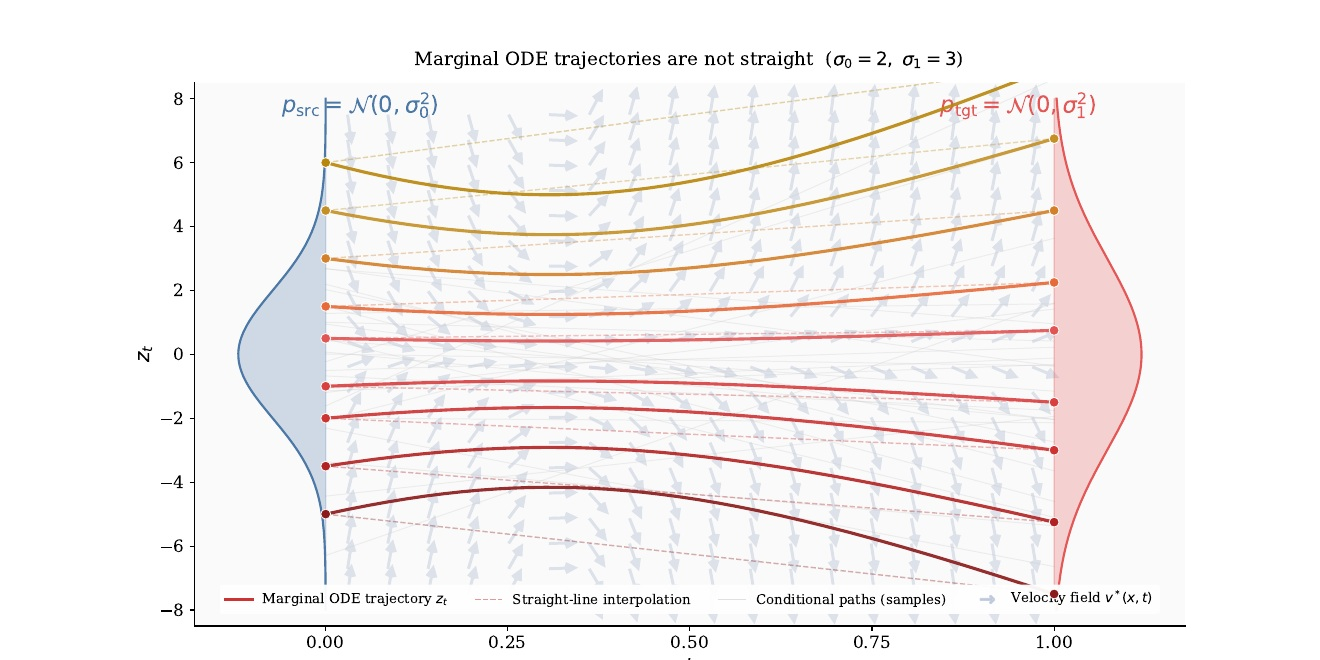
\includegraphics[width=\textwidth,height=0.62\textheight,keepaspectratio]{fig-5-10.jpg}
    \vfill
    灰：条件付き直線。実線：周辺ODE。破線：端点の直線補間。\\
    実線と破線のずれが「直線でない」証拠（$\sigma_0=2,\sigma_1=3$）。
\end{frame}
%=============================================
\asmain
\begin{frame}{5.3.5 のまとめ}
    \begin{itemize}
        \item 条件付きアフィンは直線・定速でも、周辺$v^{\star}$は事後平均
        \item 事後が$(x,t)$依存なので、周辺軌跡は一般に曲がる
        \item 直線化したいならカップリング側の工夫（Reflow）が必要
    \end{itemize}
\end{frame}
%=============================================
\section{まとめ}
\asmain
\begin{frame}{区切り：5.3 全体のまとめ}
    \tableofcontents[currentsection]
\end{frame}
%=============================================
\asmain
\begin{frame}{5.3 全体のまとめ}
    \begin{enumerate}
        \item \textbf{ガウス橋}
        閉じた$p_t$と$v_t$（命題5.3.1）が雛形になる。
        \item \textbf{Path-first}
        条件付き密度を先に置き、ビーム／スポットライトを構成する。
        \item \textbf{Flow-first}
        $\Psi_{0\to t}$を先に置き、pushforwardと一意な$v_t$を得る。
        \item \textbf{比較}
        Euler／Lagrangeの出発点の違い。使いどころが異なる。
        \item \textbf{直線性}
        条件付き直線 $\neq$ 周辺ODEの直線（図5.10）。
    \end{enumerate}
\end{frame}
%=============================================
\asmain
\begin{frame}{5.3 全体のまとめ：一本の流れ}
    \begin{block}{今日の道筋}
        ガウス橋の雛形
        $\;\to\;$
        path-first / flow-first
        $\;\to\;$
        CFM目標の具体化
        $\;\to\;$
        条件付き直線と周辺直線の落差
    \end{block}
    \begin{block}{核心}
        CFMは「扱いやすい条件付き過程」を設計する工学である。\\
        密度から入るか、フローから入るかで設計の自由度が変わる。
    \end{block}
    \begin{block}{次へ（任意）}
        5.4では標準アフィンフロー$\bm{x}_t=(1-t)\bm{x}_0+t\bm{x}_1$の性質と、\\
        Reflowによる直線化を深掘りする。
    \end{block}
\end{frame}
